% Instructor handout for the Directed Acyclic Graphs lecture.
% Compile with: latexmk -pdf handout.tex   (then latexmk -c to remove auxiliary files)
\documentclass[10pt]{article}
\usepackage[letterpaper,margin=0.5in]{geometry}
\usepackage[T1]{fontenc}
\usepackage{lmodern}
\usepackage{amsmath,amssymb}
\usepackage{xcolor}
\usepackage{tabularx,booktabs}
\usepackage{enumitem}
\usepackage{tikz}
\usetikzlibrary{arrows.meta,positioning}

\definecolor{accent}{HTML}{2980B9}
\definecolor{lightaccent}{HTML}{EEF4F9}
\definecolor{treat}{HTML}{87CEEB}
\definecolor{other}{HTML}{F4A460}
\definecolor{hidden}{HTML}{D3D3D3}
\definecolor{good}{HTML}{1A7F37}
\definecolor{bad}{HTML}{B42318}

\pagestyle{empty}
\setlength{\parindent}{0pt}
\setlength{\parskip}{3pt}
\setlist{nosep,leftmargin=*}
\renewcommand{\arraystretch}{1.15}

\newcommand{\indep}{\mathrel{\perp\!\!\!\perp}}
\newcommand{\head}[1]{\par\vspace{5pt}{\color{accent}\large\bfseries #1}\par\vspace{-1pt}{\color{accent}\rule{\linewidth}{0.8pt}}\par\vspace{2pt}}
\newcommand{\sub}[1]{\par\vspace{3pt}\textbf{#1}\par}
\newcommand{\open}{{\color{good}\bfseries Open}}
\newcommand{\blocked}{{\color{bad}\bfseries Blocked}}

% Graph styles shared by the practice cards
\tikzset{
  var/.style={circle, draw=black!80, thick, minimum size=0.75cm, inner sep=0pt, font=\small\bfseries},
  dy/.style={var, fill=treat},
  oth/.style={var, fill=other},
  hid/.style={var, fill=hidden, dashed},
  arr/.style={-{Stealth[length=2.2mm]}, thick, black!80},
}
% Mind-map styles
\tikzset{
  center/.style={rectangle, rounded corners=6pt, fill=accent, text=white, font=\bfseries\large, align=center, inner sep=8pt},
  branch/.style={rectangle, rounded corners=5pt, draw=accent, thick, fill=lightaccent, font=\small, align=center, inner sep=5pt},
  leaf/.style={rectangle, rounded corners=5pt, draw=accent!50, thick, fill=white, font=\footnotesize, align=center, inner sep=4pt},
  link/.style={rectangle, rounded corners=5pt, draw=black!35, thick, dashed, fill=black!2, font=\footnotesize, align=center, inner sep=4pt},
  line/.style={accent, thick},
  xlink/.style={black!40, thick, dashed},
  eg/.style={},
}
\newcommand{\eg}[1]{{\color{black!60}\itshape e.g.\ #1}}

\begin{document}

% ---------------------------------------------------------------- Page 1: cheat sheet
{\LARGE\bfseries Directed acyclic graphs at a glance}\par
{\color{black!60}\small Lecture reminder \textperiodcentered{} Measure Impact \textperiodcentered{} \textit{Causal Inference: The Mixtape}, Chapter 3}\par
\vspace{4pt}

\small
\begin{minipage}[t]{0.47\textwidth}
\head{The backdoor criterion}
\fcolorbox{accent}{lightaccent}{\parbox{\dimexpr\linewidth-2\fboxsep-2\fboxrule}{
A set of variables $Z$ satisfies the backdoor criterion relative to $(D, Y)$ if:
\begin{enumerate}
  \item No variable in $Z$ is a descendant of $D$
  \item $Z$ blocks every backdoor path from $D$ to $Y$
\end{enumerate}
\vspace{2pt}
Then treatment is as good as random within $Z$, the conditional independence assumption from the matching lecture:\par\centering $(Y^1, Y^0) \indep D \mid Z$}}\par\vspace{3pt}

\textbf{Why condition 1?} Conditioning on a mediator blocks part of the effect. Conditioning on any descendant of $D$ can open a collider path that starts at $D$.

\textbf{Why it matters.} The naive comparison picks up association from every open path. Open backdoor paths are the baseline bias $E[Y^0 \mid D{=}1] - E[Y^0 \mid D{=}0]$.

\textbf{Sufficient, not necessary.} If no observed set works, use randomization, an instrument, or the front-door criterion.

\head{When is a path blocked?}
\begin{tabularx}{\linewidth}{@{}lXll@{}}
\toprule
Shape & Structure & Left alone & Conditioned on \\
\midrule
Chain & $D \to M \to Y$ & \open & \blocked \\
Fork & $D \leftarrow X \to Y$ & \open & \blocked \\
Collider & $D \to C \leftarrow Y$ & \blocked & \open \\
\bottomrule
\end{tabularx}

A node blocks a path if it is a \textbf{chain or fork that we condition on}, or a \textbf{collider that we leave alone} (with none of its descendants conditioned on). One blocking node closes the whole path.
\begin{itemize}
  \item Roles belong to paths, not variables: one node can be a chain on one path and a collider on another.
  \item Colliders close long paths. Paths of only chains and forks stay open until we condition on one node.
  \item More controls are not automatically safer.
\end{itemize}

\head{Checklist}
\begin{enumerate}
  \item List every path between $D$ and $Y$, ignoring arrow direction
  \item Mark the backdoor paths (first arrow points into $D$)
  \item Note whether each is open or blocked with nothing conditioned on
  \item Find sets that block every backdoor path without opening one through a collider
  \item Drop any set that contains a descendant of $D$
\end{enumerate}

\head{The lecture's examples}
\begin{tabularx}{\linewidth}{@{}lX@{}}
\toprule
Example & Lesson \\
\midrule
Education & Condition on observed background $F$, but unobserved ability $A$ leaves a path open \\
M-bias & Pre-treatment collider: $\{\}$ is fine, $\{C\}$ opens the path, $\{A, C\}$ closes it again \\
Discrimination & Occupation is mediator and collider: direct effect not identified \\
Police & Sample selection is conditioning: $r$ falls from 0.22 to 0.12 \\
\bottomrule
\end{tabularx}
\end{minipage}\hfill
\begin{minipage}[t]{0.49\textwidth}
\head{Vocabulary}
\sub{The graph}
\begin{tabularx}{\linewidth}{@{}lX@{}}
\toprule
Term & \textit{A graph element that \dots} \\
\midrule
Node & stands for a random variable \\
Arrow & claims that one variable directly causes another \\
Missing arrow & claims that one variable does not directly cause another \\
\bottomrule
\end{tabularx}

\sub{Nodes}
\begin{tabularx}{\linewidth}{@{}lX@{}}
\toprule
Term & \textit{A node that \dots} \\
\midrule
Treatment $D$ & causes the effect we want to learn \\
Outcome $Y$ & shows the effect we measure \\
Parent of $B$ & has an arrow pointing into $B$ \\
Child of $A$ & receives an arrow from $A$ \\
Ancestor of $B$ & can reach $B$ by following arrows forward \\
Descendant of $A$ & can be reached from $A$ by following arrows forward \\
Observed & is measured in the data (solid border) \\
Unobserved & is not measured (dashed border) \\
Conditioned on & we hold fixed by comparing units with the same value (boxed) \\
Confounder & causes both $D$ and $Y$, directly or through other nodes, without passing through $D$ \\
Mediator & lies on a causal path from $D$ to $Y$ \\
\bottomrule
\end{tabularx}

\sub{Paths}
\begin{tabularx}{\linewidth}{@{}lXl@{}}
\toprule
Term & \textit{A path that \dots} & Example \\
\midrule
Path & connects two nodes through arrows, whatever their direction & $D \leftarrow X \to Y$ \\
Causal path & runs from $D$ to $Y$, every arrow pointing toward $Y$ & $D \to Y$ \\
Backdoor path & connects $D$ and $Y$ and starts with an arrow into $D$ & $D \leftarrow X \to Y$ \\
Chain at $M$ & passes through $M$, one arrow in and one out & $D \to M \to Y$ \\
Fork at $X$ & leaves $X$ along both of its arrows & $D \leftarrow X \to Y$ \\
Collider at $C$ & enters $C$ along both of its arrows & $D \to C \leftarrow Y$ \\
Open path & transmits association between its end points & \\
Blocked path & does not transmit association & \\
\bottomrule
\end{tabularx}

{\color{black!65}Chains, forks, and colliders can occur at any node along a longer path, not only between $D$ and $Y$.}

\head{Conditioning: the tool we control}
Compare $D$ and $Y$ only among units with the same value of $Z$. It takes four forms: stratifying, matching, restricting the sample, and adding a regression control. It closes chains and forks and opens colliders.

{\color{black!65}Confounder and mediator describe a variable. Chain, fork, and collider describe how one path passes through it.}
\end{minipage}

% ---------------------------------------------------------------- Page 2: mind map
\newpage
{\LARGE\bfseries The argument at a glance}\par
{\color{black!60}\small Solid lines follow the lecture's argument. Dashed boxes and lines connect it to other ideas and lectures.}\par
\vspace{18pt}

\begin{center}
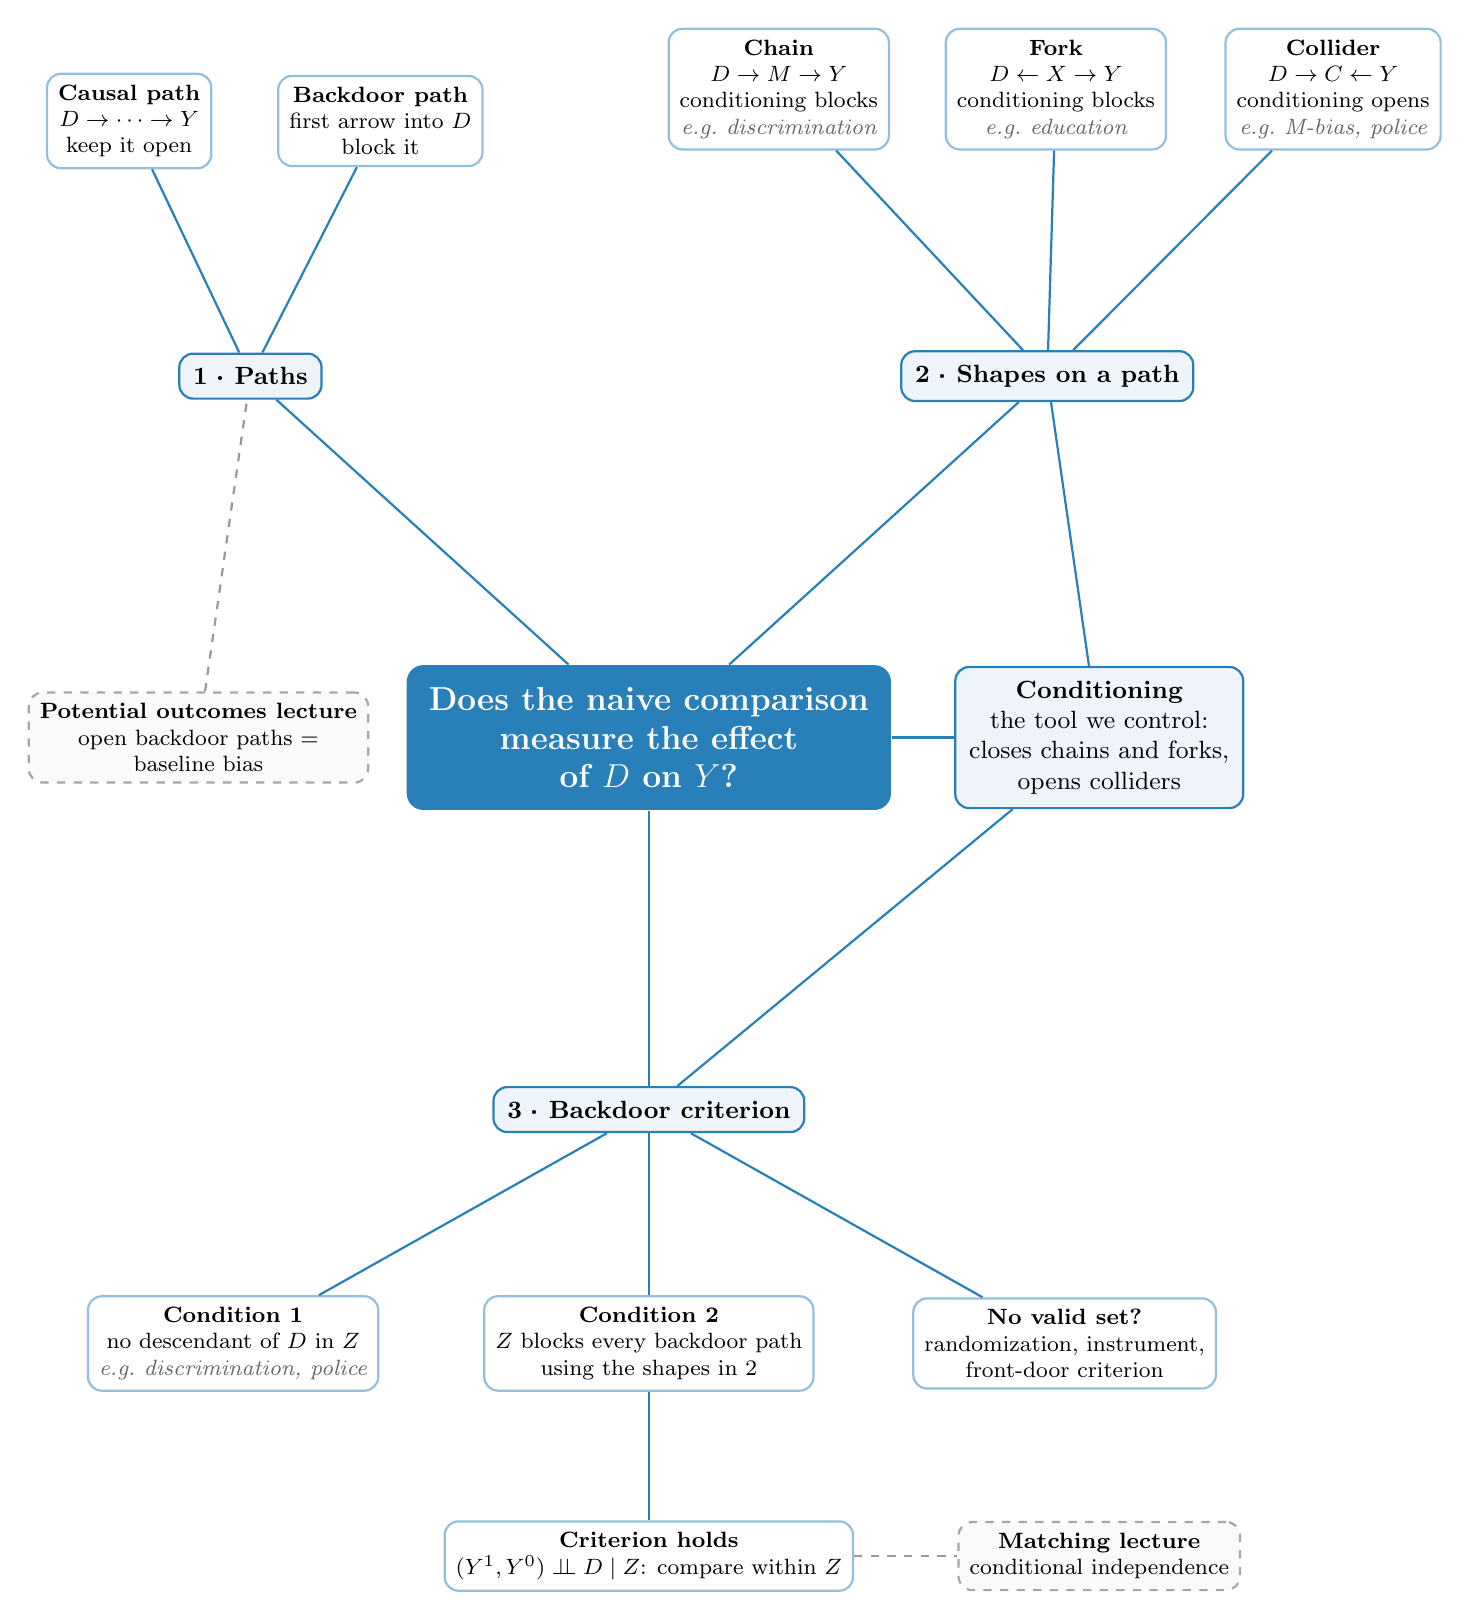
\begin{tikzpicture}[x=2.2cm, y=2.7cm]
  \node[center] (q) at (0, 0) {Does the naive comparison\\measure the effect\\of $D$ on $Y$?};

  \node[branch] (paths) at (-2.3, 1.7) {\bfseries 1 \textperiodcentered{} Paths};
  \node[leaf] (causal) at (-3.0, 2.9) {\bfseries Causal path\\$D \to \dots \to Y$\\keep it open};
  \node[leaf] (back) at (-1.55, 2.9) {\bfseries Backdoor path\\first arrow into $D$\\block it};

  \node[branch] (shapes) at (2.3, 1.7) {\bfseries 2 \textperiodcentered{} Shapes on a path};
  \node[leaf] (chain) at (0.75, 3.05) {\bfseries Chain\\$D \to M \to Y$\\conditioning blocks\\\eg{discrimination}};
  \node[leaf] (fork) at (2.35, 3.05) {\bfseries Fork\\$D \leftarrow X \to Y$\\conditioning blocks\\\eg{education}};
  \node[leaf] (coll) at (3.95, 3.05) {\bfseries Collider\\$D \to C \leftarrow Y$\\conditioning opens\\\eg{M-bias, police}};

  \node[branch] (cond) at (2.6, 0) {\bfseries Conditioning\\the tool we control:\\closes chains and forks,\\opens colliders};

  \node[branch] (crit) at (0, -1.75) {\bfseries 3 \textperiodcentered{} Backdoor criterion};
  \node[leaf] (c1) at (-2.4, -2.85) {\bfseries Condition 1\\no descendant of $D$ in $Z$\\\eg{discrimination, police}};
  \node[leaf] (c2) at (0, -2.85) {\bfseries Condition 2\\$Z$ blocks every backdoor path\\using the shapes in 2};
  \node[leaf] (none) at (2.4, -2.85) {\bfseries No valid set?\\randomization, instrument,\\front-door criterion};
  \node[leaf] (holds) at (0, -3.85) {\bfseries Criterion holds\\$(Y^1, Y^0) \indep D \mid Z$: compare within $Z$};

  \node[link] (po) at (-2.6, 0) {\bfseries Potential outcomes lecture\\open backdoor paths =\\baseline bias};
  \node[link] (match) at (2.6, -3.85) {\bfseries Matching lecture\\conditional independence};

  \draw[line] (q) -- (paths);
  \draw[line] (q) -- (shapes);
  \draw[line] (q) -- (cond);
  \draw[line] (q) -- (crit);
  \draw[line] (paths) -- (causal);
  \draw[line] (paths) -- (back);
  \draw[line] (shapes) -- (chain);
  \draw[line] (shapes) -- (fork);
  \draw[line] (shapes) -- (coll);
  \draw[line] (cond) -- (shapes);
  \draw[line] (cond) -- (crit);
  \draw[line] (crit) -- (c1);
  \draw[line] (crit) -- (c2);
  \draw[line] (crit) -- (none);
  \draw[line] (c2) -- (holds);
  \draw[xlink] (po) -- (paths);
  \draw[xlink] (holds) -- (match);
\end{tikzpicture}
\end{center}

% ---------------------------------------------------------------- Page 3: practice graphs
\newpage
{\LARGE\bfseries Practice graphs}\par
{\color{black!60}\small For each graph: which sets of observed variables satisfy the backdoor criterion for the effect of $D$ on $Y$? Dashed nodes are unobserved.}\par
\vspace{6pt}

% Coordinates follow the practice-card figures (x right, y down, in figure pixels)
\tikzset{card/.style={x=0.0125cm, y=-0.0125cm}}
\newcommand{\card}[3]{%
  \begin{minipage}[t]{0.49\textwidth}
  \fcolorbox{black!25}{white}{\parbox{\dimexpr\linewidth-2\fboxsep-2\fboxrule}{%
    {\color{accent}\bfseries #1}\par
    \centering\begin{tikzpicture}[card]#2\end{tikzpicture}\par
    \raggedright\small #3}}
  \end{minipage}}

\card{Card 1}{
  \node[dy] (D) at (90,190) {D}; \node[dy] (Y) at (450,190) {Y}; \node[oth] (X) at (270,60) {X};
  \draw[arr] (X) -- (D); \draw[arr] (X) -- (Y); \draw[arr] (D) -- (Y);
}{Which sets satisfy the backdoor criterion?}\hfill
\card{Card 2}{
  \node[dy] (D) at (90,190) {D}; \node[oth] (M) at (270,60) {M}; \node[dy] (Y) at (450,190) {Y};
  \draw[arr] (D) -- (M); \draw[arr] (M) -- (Y); \draw[arr] (D) -- (Y);
}{Which sets satisfy the backdoor criterion?}

\vspace{8pt}
\card{Card 3}{
  \node[oth] (B) at (270,50) {B}; \node[oth] (A) at (90,120) {A}; \node[dy] (D) at (90,240) {D}; \node[dy] (Y) at (450,240) {Y};
  \draw[arr] (B) -- (A); \draw[arr] (A) -- (D); \draw[arr] (B) -- (Y); \draw[arr] (D) -- (Y);
}{Which sets satisfy the criterion? Bonus: is there more than one valid set?}\hfill
\card{Card 4}{
  \node[oth] (A) at (90,50) {A}; \node[oth] (B) at (450,50) {B}; \node[oth] (C) at (270,140) {C};
  \node[dy] (D) at (90,240) {D}; \node[dy] (Y) at (450,240) {Y};
  \draw[arr] (A) -- (D); \draw[arr] (A) -- (C); \draw[arr] (B) -- (C); \draw[arr] (B) -- (Y); \draw[arr] (D) -- (Y);
}{Which sets satisfy the backdoor criterion?}

\vspace{8pt}
\card{Card 5}{
  \node[oth] (X) at (270,50) {X}; \node[dy] (D) at (90,150) {D}; \node[dy] (Y) at (450,150) {Y}; \node[oth] (C) at (270,250) {C};
  \draw[arr] (X) -- (D); \draw[arr] (X) -- (Y); \draw[arr] (D) -- (Y); \draw[arr] (D) -- (C); \draw[arr] (Y) -- (C);
}{Which sets satisfy the backdoor criterion?}\hfill
\card{Card 6}{
  \node[hid] (U) at (270,50) {U}; \node[oth] (X) at (90,120) {X}; \node[dy] (D) at (90,240) {D}; \node[dy] (Y) at (450,240) {Y};
  \draw[arr] (U) -- (X); \draw[arr] (X) -- (D); \draw[arr] (U) -- (Y); \draw[arr] (D) -- (Y);
}{Which sets satisfy the criterion? $U$ is unobserved.}

\vspace{8pt}
\card{Card 7}{
  \node[oth] (A) at (90,50) {A}; \node[oth] (B) at (450,50) {B}; \node[oth] (C) at (270,140) {C};
  \node[dy] (D) at (90,240) {D}; \node[dy] (Y) at (450,240) {Y};
  \draw[arr] (A) -- (D); \draw[arr] (A) -- (C); \draw[arr] (B) -- (C); \draw[arr] (B) -- (Y);
  \draw[arr] (C) -- (D); \draw[arr] (C) -- (Y); \draw[arr] (D) -- (Y);
}{Which sets satisfy the criterion? Bonus: is $C$ a confounder, a collider, or both?}\hfill
\card{Card 8}{
  \node[dy] (D) at (90,240) {D}; \node[oth] (M) at (270,90) {M}; \node[dy] (Y) at (450,240) {Y}; \node[hid] (U) at (450,60) {U};
  \draw[arr] (D) -- (M); \draw[arr] (M) -- (Y); \draw[arr] (D) -- (Y); \draw[arr] (U) -- (M); \draw[arr] (U) -- (Y);
}{$U$ is unobserved. Answer for the total effect, then for the direct effect not via $M$.}

% ---------------------------------------------------------------- Page 4: answers
\newpage
{\LARGE\bfseries Practice graphs: answers}\par
\vspace{6pt}
\small
\begin{tabularx}{\textwidth}{@{}l>{\raggedright\arraybackslash}p{3.3cm}X@{}}
\toprule
Card & Valid sets & Why \\
\midrule
1 & $\{X\}$ & Conditioning on the fork $X$ blocks the only backdoor path, the basic confounding case. \\
2 & $\{\}$ & No backdoor path, so the naive comparison identifies the total effect. $M$ is a descendant of $D$, so the criterion rules it out; conditioning on it would block part of the effect. \\
3 & $\{A\}$, $\{B\}$, $\{A, B\}$ & The backdoor path $D \leftarrow A \leftarrow B \to Y$ has no collider. One blocked node closes it, so $A$ or $B$ is enough. $A$ is a valid control although it is not a confounder. \\
4 & $\{\}$, $\{A\}$, $\{B\}$, $\{A, B\}$, $\{A, C\}$, $\{B, C\}$, $\{A, B, C\}$ & M-bias. The collider $C$ already blocks the backdoor path. Only $\{C\}$ fails, because it opens the path; adding $A$ or $B$ closes it again. \\
5 & $\{X\}$ & $D \to C \leftarrow Y$ starts with an arrow out of $D$, so condition 2 ignores it, but condition 1 rules out $C$ as a descendant of $D$. Conditioning on $C$ would open that path. \\
6 & $\{X\}$ & The confounder $U$ is unobserved, but blocking $D \leftarrow X \leftarrow U \to Y$ at the observed chain node $X$ is enough. \\
7 & $\{A, C\}$, $\{B, C\}$, $\{A, B, C\}$ & $C$ is both a confounder and a collider. $D \leftarrow C \to Y$ can only be blocked at $C$, which opens $D \leftarrow A \to C \leftarrow B \to Y$, so $A$ or $B$ must close it. Neither $\{C\}$ nor $\{A, B\}$ works. \\
8 & $\{\}$ & No backdoor path, so the naive comparison identifies the total effect. For the direct effect, conditioning on $M$ blocks $D \to M \to Y$ but opens $D \to M \leftarrow U \to Y$; with $U$ unobserved, no set identifies it. This is the discrimination example. \\
\bottomrule
\end{tabularx}

\end{document}
